\nnarticleheader{\emph{How to Solve It} and the Bear Riddle}{Mitav Nayak, Haverford '22}

\noindent
\textbf{Introduction}

The riddle in this article was taken from \emph{How to Solve It}, a famous book describing the mathematical method by George Pólya. It was published in 1945, and it describes four steps one can take when problem solving:

\begin{enumerate}
   \item Understanding the Problem
   \begin{itemize}
     \item Here, you may have to identify the unknown, conditions, and data, draw a figure, and introduce notation.
   \end{itemize}
   \item Devising a Plan
   \begin{itemize}
     \item Next, you examine a connection between the data and the unknown. You may consider a similar problem to devise your plan.
   \end{itemize}
   \item Carrying Out the Plan
   \begin{itemize}
     \item The next step is to carry out your plan, checking each step as you work through the problem.
   \end{itemize}
   \item Looking Back
   \begin{itemize}
     \item Finally, check your final answer. You may consider using a different method to derive the same result.
   \end{itemize}
\end{enumerate}

\noindent
We will now use Polya’s steps on a classic brainteaser.

\noindent
\textbf{The Problem}

A bear, starting from the point \emph{P}, walked one mile due south. Then he changed direction and walked one mile due east. Then he turned again to the left and walked one mile due north, and arrived exactly at the point \emph{P} he started from. What was the color of the bear?

\noindent
\textbf{The Explanation}

After looking at this problem, we may be initially confused. Firstly, how can a bear walk one mile south, one mile east, and one mile north, and end up at the same point he started? Secondly, how does this pertain to the color of the bear? Let’s break the problem down into the four steps.

\begin{enumerate}
   \item Understanding the Problem
  
   While the first question posed will be important in the solution, it is not the unknown. Rather, the unknown is the color of the bear. The bear’s travel and directions traveled are data, not the unknown.
   
   To understand the problem, we can also draw a figure:
   
   \vspace{1cm}
   
   \renewcommand{\thefigure}{1}
   \begin{figure}[htp]
    \centering
    \begin{minipage}{6cm}
    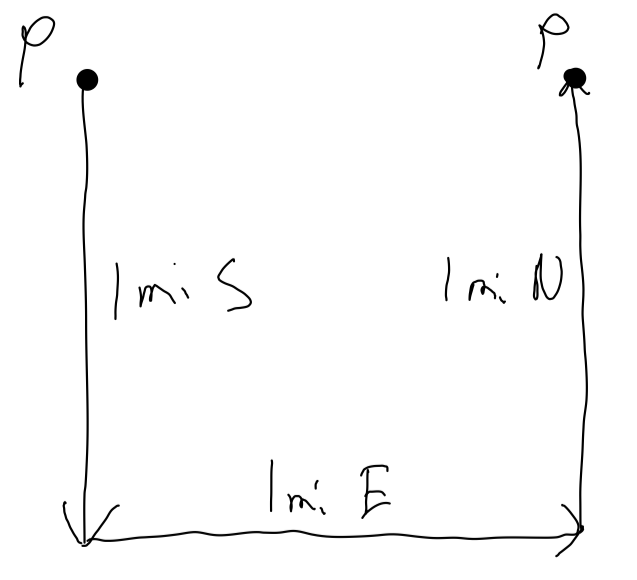
\includegraphics[width=6cm]{nayakb_image1}
    \caption{An initial attempt at drawing a figure.}
    \label{fig:1}
    \end{minipage}
\end{figure}

\pagebreak
   \item Devising a Plan
   
   If we have seen a similar problem we may consider that. If not, we can try to connect the data to the unknown. We can pose the following questions:
   
   \begin{itemize}
     \item Where do bears live? What are some colors bears may be?
     \item Where on the earth may a bear be able to walk south, east, and north, and end up at the same spot?
   \end{itemize}
   
   After some thought, we realize that the solution may pertain to a specific location on the earth, since the color of a bear varies depending on its location. Also, the earth is spherical, so our figure would look quite different if we were at some locations on the earth. Our plan may be to draw more figures, each at different points on the earth.
   
   \item Carrying Out the Plan
   
   \renewcommand{\thefigure}{2}
\begin{figure}[!htb]
   \begin{minipage}{0.48\textwidth}
     \centering
     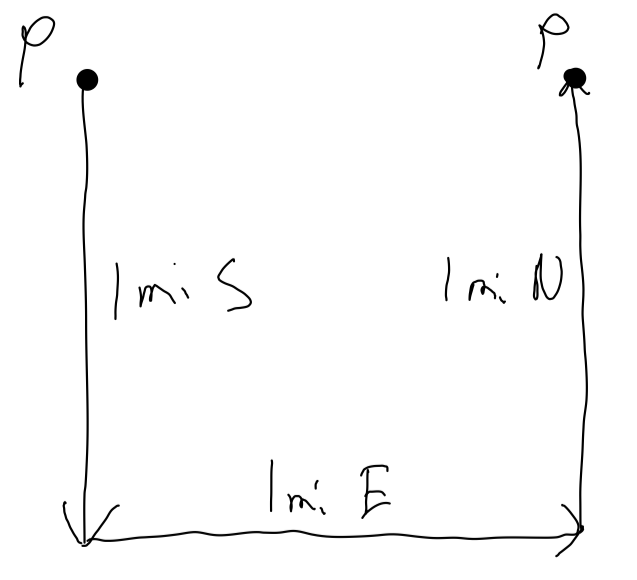
\includegraphics[width=.9\linewidth]{nayakb_image1}
     \caption{A general illustration of the problem.}\label{Fig:1}
   \end{minipage}\hfill
   \begin{minipage}{0.48\textwidth}
     \centering
     \renewcommand{\thefigure}{3}
     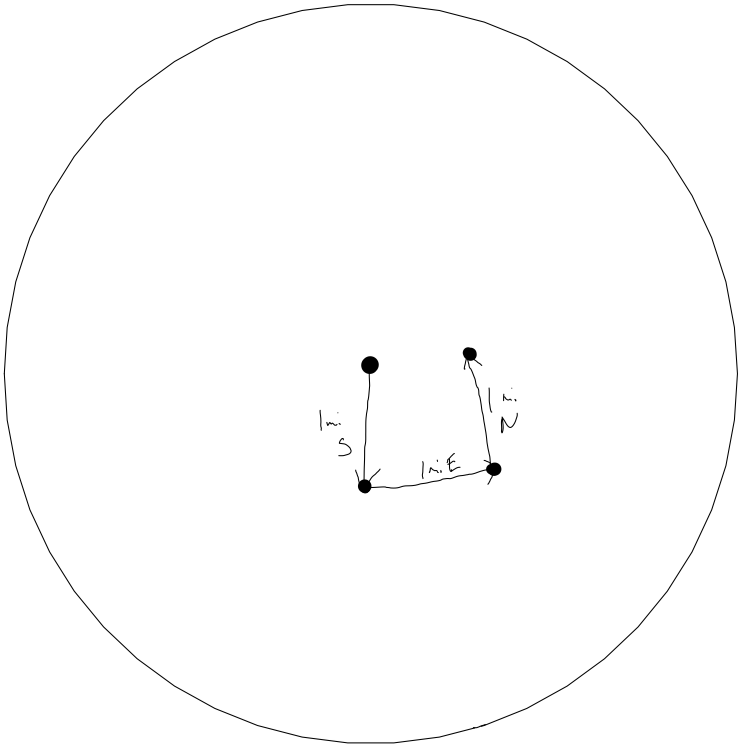
\includegraphics[width=.9\linewidth]{nayakb_image2}
     \caption{Point \emph{P} is near the equator.}\label{Fig:2}
   \end{minipage}
\end{figure}

\renewcommand{\thefigure}{4}
\begin{figure}[!htb]
   \begin{minipage}{0.48\textwidth}
     \centering
     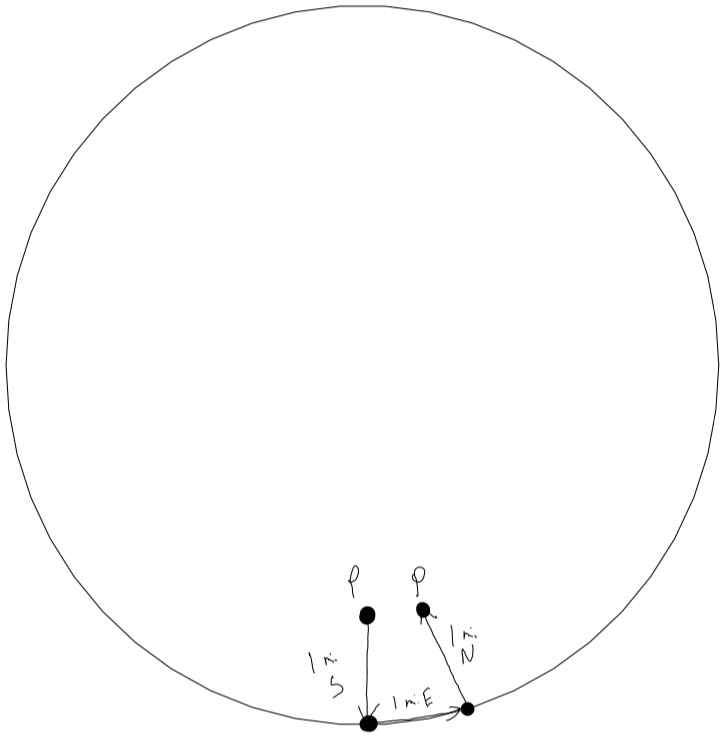
\includegraphics[width=.9\linewidth]{nayakb_image3}
     \caption{Point \emph{P} is 1 mile north of the South Pole.}\label{Fig:Data1}
   \end{minipage}\hfill
   \begin{minipage}{0.48\textwidth}
     \centering
     \renewcommand{\thefigure}{5}
     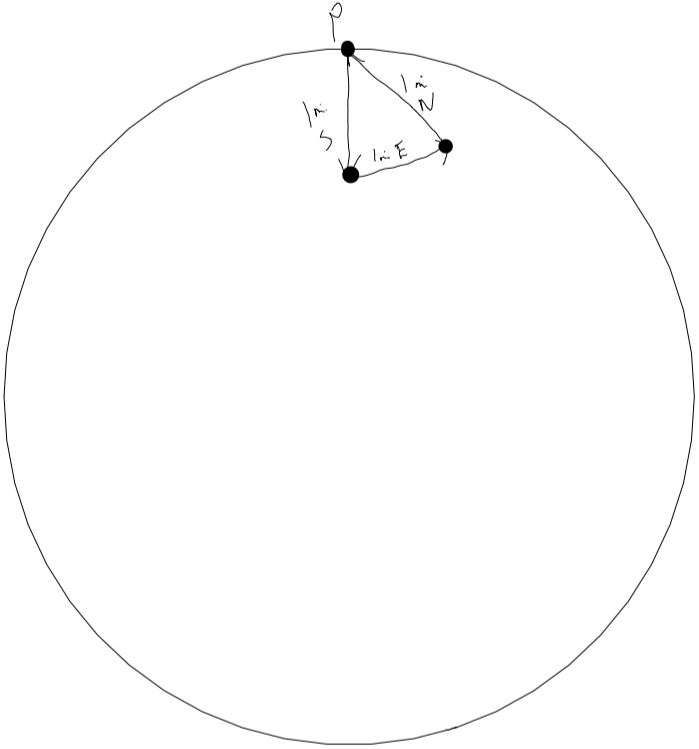
\includegraphics[width=.9\linewidth]{nayakb_image4}
     \caption{Point \emph{P} is at the North Pole.}\label{Fig:Data2}
   \end{minipage}
\end{figure}


\pagebreak
   Based on our North Pole figure, we have found where it may be possible for the bear to end up at the same point. We know that bears at the North Pole are white, and this is our answer to the riddle.

 
   
   \item Looking Back
   
   We can check our figure again. If we assume the globe is a perfect sphere, and the bear moves due south, due east, and due north, it will indeed end at the same place it began: the North Pole.
   
\end{enumerate}


\begin{thebibliography}{1}

\bibitem{} 
Polya, George. How to Solve It. Princeton University Pres, 2009.

\end{thebibliography}
